% Section 5: Direct Sums and Orthogonal Projections  (original handwritten pages 33--42)
\section{Direct Sums and Orthogonal Projections}\label{sec:direct-sum}
\syllabusweek{Week 6 --- direct sum decompositions, projection theorem, orthogonal projections}

\subsection{Direct Sums}\label{ss:direct-sums}

\begin{definition}
Let $\V$ be a vector space and let $M_1,\dots,M_k$ be subspaces of $\V$. The \term{sum} of these subspaces is defined as
\[
M=M_1+M_2+\dots+M_k=\{m\in\V \mid m=m_1+m_2+\dots+m_k,\ m_i\in M_i\ \forall i\}.
\]
The subspaces are called \term{linearly independent} iff
\[
m_1+m_2+\dots+m_k=0_V \quad\text{where } m_i\in M_i\ \forall i
\quad\Rightarrow\quad m_1=m_2=\dots=m_k=0_V .
\]
\end{definition}

\begin{center}
\begin{minipage}{0.42\textwidth}\centering
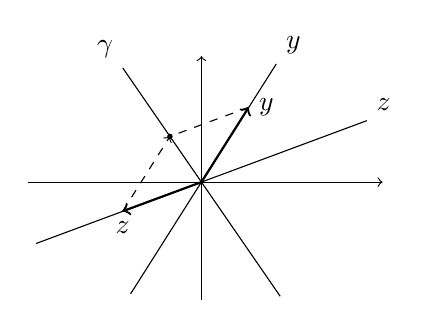
\begin{tikzpicture}[scale=1.0]
% axes
\draw[->] (-2.2,0) -- (2.3,0);
\draw[->] (0,-1.5) -- (0,1.6);
% subspaces (lines through the origin)
\draw (-0.9,-1.42) -- (0.95,1.5) node[above right] {$y$};
\draw (-2.1,-0.78) -- (2.1,0.78) node[above right] {$z$};
\draw (-1.0,1.45) -- (1.0,-1.45);
\node[above left] at (-1.0,1.45) {$\gamma$};
% vectors y, z and y+z = gamma
\draw[->,thick] (0,0) -- (0.6,0.95) node[right] {$y$};
\draw[->,thick] (0,0) -- (-1.0,-0.37) node[below] {$z$};
\draw[->,dashed] (-1.0,-0.37) -- (-0.4,0.58);
\draw[dashed] (0.6,0.95) -- (-0.4,0.58);
\fill (-0.4,0.58) circle (1pt);
\end{tikzpicture}
\end{minipage}%
\begin{minipage}{0.4\textwidth}
$y+z-\gamma=0$\\
$\Rightarrow$ not linearly independent
\end{minipage}
\end{center}

% ===== Page 33 =====
\begin{remark}\leavevmode\origpage{33}
Let $\V=M_1+M_2+\dots+M_k$ and let $M_1,\dots,M_k$ be linearly independent. Then for $x\in\V$,
\[
x=m_1+m_2+\dots+m_k, \qquad m_i\in M_i\ \forall i,
\]
\key{$m_1,m_2,\dots,m_k$ are unique.}
\end{remark}

\begin{proof}
Assume $m_1,\dots,m_k$ are not unique, i.e.\ there is an $i$ such that $m_i\ne\bar m_i$:
\begin{align*}
x&=m_1+\dots+m_k\\
x&=\bar m_1+\dots+\bar m_k\\
0_V&=\underbrace{(m_1-\bar m_1)}_{\in M_1}+\underbrace{(m_2-\bar m_2)}_{\in M_2}+\dots+\underbrace{(m_k-\bar m_k)}_{\in M_k}
\end{align*}
$\Rightarrow M_1,\dots,M_k$ are not linearly independent. \qedhere
\end{proof}

\begin{definition}
Let $M_1,\dots,M_k$ be subspaces of $\V$. Let
\begin{enumerate}[label=\roman*-)]
\item $M=M_1+M_2+\dots+M_k$.
\item $M_1,M_2,\dots,M_k$ are linearly independent.
\end{enumerate}
Then $M$ is said to be the \term{direct sum} of $M_1,\dots,M_k$. This is shown as
\[
M=M_1\oplus M_2\oplus\dots\oplus M_k .
\]
\end{definition}

\begin{example}
$\V=\R^4$, \quad $x=(x_1,x_2,x_3,x_4)^T\in\R^4$.
\begin{alignat*}{3}
M_1&\triangleq\{x\in\R^4\mid x_4=x_3=0\}: &\quad &\bmat{x_1\\x_2\\0\\0}, &\quad \dim&=2\\
M_2&\triangleq\{x\in\R^4\mid x_1=x_2=0\}: & &\bmat{0\\0\\x_3\\x_4}, & \dim&=2\\
M_3&\triangleq\{x\in\R^4\mid x_1=0\}: & &\bmat{0\\x_2\\x_3\\x_4}, & \dim&=3
\end{alignat*}
\begin{align*}
M_1+M_2&=\R^4 && \Rightarrow \text{direct sum: } M_1\,\&\,M_2 \text{ linearly independent} \Rightarrow M_1\oplus M_2=\R^4\\
M_1+M_3&=\R^4 && \Rightarrow \text{not direct sum}\\
M_2+M_3&=M_3 && \Rightarrow \text{not direct sum } (M_2\subset M_3)
\end{align*}

\sep
For $M_1$ and $M_3$:
\[
\bmat{x_1\\x_2\\0\\0}+\bmat{0\\x_2'\\x_3'\\x_4'}=\bmat{0\\0\\0\\0},
\qquad\text{e.g.}\qquad
\underset{\in M_1}{\bmat{0\\1\\0\\0}}+\underset{\in M_3}{\bmat{0\\-1\\0\\0}}=\underset{0_V}{\bmat{0\\0\\0\\0}}
\]
As the two summands are nonzero, $M_1\,\&\,M_3$ are linearly dependent.\\
$\therefore$ \key{$M_1+M_3$ is not a direct sum.}

$M_2\,\&\,M_3$ are linearly dependent (e.g.\ $m_2=(0,0,1,0)^T\in M_2$, $m_3=-m_2\in M_3$).\\
$\therefore$ \key{$M_2+M_3$ is not a direct sum.}
\begin{insight}[Dimension test]
For two subspaces, $M_1+M_2$ is direct $\iff M_1\cap M_2=\{0_V\}\iff\dim(M_1+M_2)=\dim M_1+\dim M_2$. Here: $M_1\cap M_2=\{0\}$ and $2+2=4$ (direct); $M_1\cap M_3=\{(0,x_2,0,0)^T\}$, $2+3=5\ne4$ (not direct); $M_2\cap M_3=M_2$, $2+3\ne3$ (not direct).
\end{insight}
\end{example}

% ===== Page 34 =====
\subsection{Orthogonal Direct Sums and Orthogonal Complements}\label{ss:orth-complement}

\begin{definition}\leavevmode\origpage{34}
Let $\V$ be an inner product space. Two subspaces $M_1\,\&\,M_2$ are said to be \term{orthogonal} iff
\[
\inner{m_1}{m_2}=0 \qquad \forall m_1\in M_1,\ \forall m_2\in M_2 .
\]
We denote this $M_1\perp M_2$.
\end{definition}
% corrected: notes had "M_2 & M_2" in the first line; M_1 & M_2 meant.

\needspace{8\baselineskip}
\begin{definition}
Let $M$ be equal to $M_1+M_2+\dots+M_k$ and $M_i\perp M_j$ for $i\ne j$. Then $M$ is said to be an \term{orthogonal direct sum} of $M_1,\dots,M_k$. We show this as
\[
M=M_1\overset{\perp}{\oplus}M_2\overset{\perp}{\oplus}\dots\overset{\perp}{\oplus}M_k .
\]
If $M=\V$ then
\[
\V=M_1\overset{\perp}{\oplus}M_2\overset{\perp}{\oplus}\dots\overset{\perp}{\oplus}M_k
\]
is called an \term{orthogonal direct sum decomposition} of $\V$.
\end{definition}

\begin{claim}
\key{Orthogonality implies linear independence.}
\end{claim}
\begin{proof}
Let $\sum_{i=1}^{k}m_i=0_V$, \ $m_i\in M_i$. Then
\begin{align*}
\Big\langle\sum_{i=1}^{k}m_i,\,m_j\Big\rangle&=\inner{0_V}{m_j}=0\\
\sum_{i=1}^{k}\inner{m_i}{m_j}&=0
\end{align*}
Since $\inner{m_i}{m_j}=0$ when $i\ne j$:
\[
\inner{m_j}{m_j}=0 \ \Rightarrow\ m_j=0_V .
\]
\explain{The last step uses positive definiteness of the inner product. Since $j$ was arbitrary, all $m_j=0_V$: orthogonality implies linear independence.}
\end{proof}

\begin{definition}
Let $M$ be a subspace of an inner product space $\V$. The \term{orthogonal complement} $M^\perp$ of the subspace is defined as
\[
M^\perp=\{x\in\V\mid \inner{x}{m}=0\ \forall m\in M\}.
\]
\end{definition}
The zero vector is orthogonal to every vector, so $0_V\in M^\perp$ always. Two examples:

\begin{center}
\begin{minipage}{0.34\textwidth}\centering
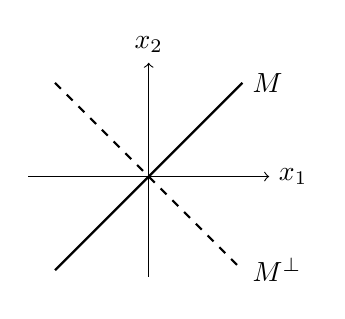
\begin{tikzpicture}[scale=0.85]
\draw[->] (-1.8,0) -- (1.8,0) node[right] {$x_1$};
\draw[->] (0,-1.5) -- (0,1.7) node[above] {$x_2$};
\draw[thick] (-1.4,-1.4) -- (1.4,1.4) node[right] {$M$};
\draw[thick,dashed] (-1.4,1.4) -- (1.4,-1.4) node[right] {$M^\perp$};
\end{tikzpicture}
\end{minipage}%
\begin{minipage}{0.6\textwidth}
\begin{align*}
M&=\Span\left\{\bmat{1\\1}\right\}, & \bmat{-1\\1}&\in M^\perp, \quad \bmat{2\\-2}\in M^\perp\\
M^\perp&=\Span\left\{\bmat{-1\\1}\right\}, & M+M^\perp&=M\overset{\perp}{\oplus}M^\perp
\end{align*}
\end{minipage}
\end{center}
\begin{center}
\begin{minipage}{0.3\textwidth}\centering
\begin{tikzpicture}[scale=0.85]
\fill[pattern=vertical lines, pattern color=gray!70] (-0.2,0) -- (2,0) -- (1.2,-1.2) -- (-1.0,-1.2) -- cycle;
\draw[->] (0,0) -- (0,2) node[above] {$z$};
\draw[->] (0,0) -- (2.3,0) node[right] {$y$};
\draw[->] (0,0) -- (-0.95,-1.45) node[below left] {$x$};
\node at (1.25,-0.75) {$M$};
\node[right] at (0,1.4) {$M^\perp$};
\end{tikzpicture}
\end{minipage}%
\begin{minipage}{0.55\textwidth}
\begin{align*}
M&=\{x\text{-}y \text{ plane}\}\\
M^\perp&=\{z \text{ axis}\}\\
\underset{\dim=2}{M}\overset{\perp}{\oplus}\underset{\dim=1}{M^\perp}&=\underset{\dim 3}{\R^3}
\end{align*}
\end{minipage}
\end{center}
Orthogonality implies linear independence, thus this is a direct sum; since the summands are also orthogonal, it is an orthogonal direct sum.

\needspace{9\baselineskip}
\begin{claim}
\key{$M^\perp$ is a subspace of $\V$.}
\end{claim}
\begin{proof}
Let $x,y\in M^\perp$, i.e.\ $\inner{x}{m}=0$, $\inner{y}{m}=0$ $\forall m\in M$. Then
\begin{align*}
\inner{x+y}{m}&=\underbrace{\inner{x}{m}+\inner{y}{m}}_{0} \quad (m\in M)\\
&=0 \quad \forall m\in M &&\Rightarrow\ x+y\in M^\perp\\
\inner{\alpha x}{m}&=\alpha\inner{x}{m}=0 \quad\forall m\in M &&\Rightarrow\ \alpha x\in M^\perp
\end{align*}
$\therefore$ $M^\perp$ is closed under addition and scalar multiplication, hence a subspace of $\V$.
\end{proof}

% ===== Page 35 =====
\begin{theorem}[Orthogonal decomposition]\leavevmode\origpage{35}
Let $\V$ be an inner product space and $M$ a subspace of $\V$. Then \key{$\V$ is the orthogonal direct sum of $M$ and $M^\perp$}:
\[
\boxed{\V=M\overset{\perp}{\oplus}M^\perp}
\]
To prove this we check:
\begin{itemize}[nosep]
\item $\V=M+M^\perp$ \ (to be shown, proof below);
\item $M\,\&\,M^\perp$ are linearly independent \ $\checkmark$;
\item $M\perp M^\perp$ \ $\checkmark$.
\end{itemize}
\end{theorem}

\begin{proof}
It remains to show $\V=M+M^\perp$.

\paragraph{Part I.} $\dim M=n\triangleq\dim\V \Rightarrow M=\V$ \ \textcircled{?}\par
\explain{Answer to \textcircled{?}: a basis of $M$ consists of $n$ linearly independent vectors of $\V$; in an $n$-dimensional space any $n$ independent vectors form a basis, so they span $\V$ and $M=\V$.}

\begin{center}
\begin{minipage}{0.25\textwidth}\centering
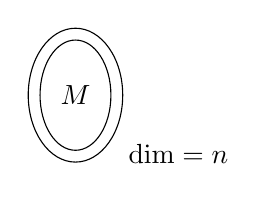
\begin{tikzpicture}
\draw (0,0) ellipse (0.6 and 0.85);
\draw (0,0) ellipse (0.45 and 0.7);
\node at (0,0) {$M$};
\node[right] at (0.55,-0.75) {$\dim\V=n$};
\end{tikzpicture}
\end{minipage}%
\begin{minipage}{0.6\textwidth}
\begin{align*}
M^\perp&=\V^\perp=\{0_V\}\\
\V&=M+M^\perp\\
x&=\underset{\in M}{x_1}+\underset{\in M^\perp}{x_2}
\ \Rightarrow\ x=\underset{\in M}{x}+\underset{\in M^\perp}{0_V} \quad\checkmark
\end{align*}
\end{minipage}
\end{center}

\paragraph{Part II.} $\dim M<n$, with $\dim M = k$. Let
\begin{align*}
B&=\{m_1,m_2,m_3,\dots,m_k\} && \text{(basis for } M)\\
C&=\{m_1,m_2,\dots,m_k,m_{k+1},\dots,m_n\} && \text{(basis for } \V)
\end{align*}
Apply Gram--Schmidt orthogonalization to $C$:
\[
\bar C=\{\underbrace{\underset{\uparrow\, m_1}{e_1},e_2,\dots,e_k}_{\text{form a basis for } M},\ \overbrace{e_{k+1},\dots,e_n}^{\text{basis for } M^\perp}\},
\qquad
\Span\{e_1,\dots,e_k\}=\Span\{m_1,\dots,m_k\}.
\]
$\bar C$ is a basis for $\V$. For $x\in\V$:
\[
x=\sum_{i=1}^{n}\alpha_ie_i=\underbrace{\sum_{i=1}^{k}\alpha_ie_i}_{x_1\in M}+\underbrace{\sum_{j=k+1}^{n}\alpha_je_j}_{x_2\in M^\perp}
\]
\explain{$x_2\in M^\perp$ by construction: Gram--Schmidt makes each $e_j$ ($j>k$) orthogonal to $e_1,\dots,e_k$, which span $M$; hence $e_j\perp m$ for all $m\in M$, and so is every combination of them.}
\[
\Rightarrow\ x=\underset{\in M}{x_1}+\underset{\in M^\perp}{x_2}\ \Rightarrow\ \V=M+M^\perp \qedhere
\]
\end{proof}
\begin{insight}[The remaining two items]
The other two items are immediate: $M\perp M^\perp$ by the definition of $M^\perp$, and orthogonality implies linear independence (shown above), equivalently $M\cap M^\perp=\{0_V\}$ since $x\in M\cap M^\perp\Rightarrow\inner{x}{x}=0$. Consequently $\dim M^\perp=\dim\V-\dim M$, and $\{e_{k+1},\dots,e_n\}$ is in fact a basis of $M^\perp$. (Finite dimension of $\V$ is assumed in the proof.)
\end{insight}

\begin{example}
$\V=\R^4$,
\[
M=\Span\left\{\bmat{1\\2\\3\\4},\bmat{4\\3\\2\\1}\right\}. \qquad \text{Find a basis for } M^\perp.
\]
Complete the basis of $M$ with two canonical vectors to a basis of $\R^4$ and orthogonalize:
\[
C=\Big\{\underset{m_1}{\bmat{1\\2\\3\\4}},\ \underset{m_2}{\bmat{4\\3\\2\\1}},\ \underset{m_3}{\bmat{1\\0\\0\\0}},\ \underset{m_4}{\bmat{0\\1\\0\\0}}\Big\}
\ \xrightarrow{\text{Gram--Schmidt}}\ \bar C=\{e_1,e_2,e_3,e_4\}
\]
% corrected: notes labelled the un-orthogonalized vectors [1,0,0,0], [0,1,0,0] themselves as e_3, e_4 and wrote M^perp = sp{e_3,e_4};
% these vectors are NOT orthogonal to M (e.g. <[1,0,0,0],m_1> = 1). The last vector is cramped in the scan (could be read as 0,1,3);
% [0,1,0,0] is the reading used. The Gram--Schmidt computation below is added and verified with exact (Fraction) arithmetic.
\begin{align*}
e_1&=m_1=\bmat{1\\2\\3\\4}, \qquad \inner{e_1}{e_1}=30\\
e_2&=m_2-\frac{\inner{m_2}{e_1}}{\inner{e_1}{e_1}}e_1=\bmat{4\\3\\2\\1}-\frac{20}{30}\bmat{1\\2\\3\\4}=\frac53\bmat{2\\1\\0\\-1}\ \to\ \bmat{2\\1\\0\\-1}\\
e_3&=m_3-\frac{\inner{m_3}{e_1}}{\inner{e_1}{e_1}}e_1-\frac{\inner{m_3}{e_2}}{\inner{e_2}{e_2}}e_2
 =\bmat{1\\0\\0\\0}-\frac{1}{30}\bmat{1\\2\\3\\4}-\frac{2}{6}\bmat{2\\1\\0\\-1}=\frac1{10}\bmat{3\\-4\\-1\\2}\ \to\ \bmat{3\\-4\\-1\\2}\\
e_4&=m_4-\frac{\inner{m_4}{e_1}}{\inner{e_1}{e_1}}e_1-\frac{\inner{m_4}{e_2}}{\inner{e_2}{e_2}}e_2-\frac{\inner{m_4}{e_3}}{\inner{e_3}{e_3}}e_3\\
 &=\bmat{0\\1\\0\\0}-\frac{2}{30}\bmat{1\\2\\3\\4}-\frac{1}{6}\bmat{2\\1\\0\\-1}+\frac{4}{30}\bmat{3\\-4\\-1\\2}=\frac16\bmat{0\\1\\-2\\1}\ \to\ \bmat{0\\1\\-2\\1}
\end{align*}
\explain{Scaling a vector does not affect orthogonality, so after each step the vector is rescaled to integer entries ($\to$) and the scaled version is used in the following steps.}
\[
\boxed{M^\perp=\Span\{e_3,e_4\}=\Span\left\{\bmat{3\\-4\\-1\\2},\bmat{0\\1\\-2\\1}\right\}}
\]
\begin{insight}[Verification]
$\inner{e_3}{m_1}=3-8-3+8=0$, \ $\inner{e_3}{m_2}=12-12-2+2=0$, \ $\inner{e_4}{m_1}=2-6+4=0$, \ $\inner{e_4}{m_2}=3-4+1=0$, \ and $\inner{e_3}{e_4}=-4+2+2=0$. Since $e_3,e_4\ne0$, the set $C$ was indeed a basis of $\R^4$.

Alternatively,
\[
x\in M^\perp\iff\bmat{1&2&3&4\\4&3&2&1}x=0, \qquad\text{i.e.}\qquad M^\perp=\Null\!\left(\bmat{1&2&3&4\\4&3&2&1}\right),
\]
which has dimension $4-2=2$ and is spanned e.g.\ by $(1,-2,1,0)^T$ and $(0,1,-2,1)^T$; note $(3,-4,-1,2)^T=3(1,-2,1,0)^T+2(0,1,-2,1)^T$, so both answers describe the same subspace. Gram--Schmidt additionally gives an \emph{orthogonal} basis.
\end{insight}
\end{example}

% ===== Page 36 =====
\subsection{The Projection Theorem}\label{ss:projection-thm}
\begin{theorem}[Hilbert's Projection Theorem]
Let $H$ be a Hilbert space\origpage{36} and let $M$ be a finite dimensional subspace of $H$.
For any $x\in H$ the following minimization problem has a solution:
\[
m^* = \arg\min_{m\in M} \norm{x-m}^{2}
\]
\begin{itemize}[nosep]
  \item the exponent $2$ does not matter, the norm is positive;
  \item $\norm{\cdot}$ is the norm induced by the inner product.
\end{itemize}
In other words, we can find the closest vector $m^*$ to $x$ lying in the subspace $M$.
If $m^*$ is a solution, then \key{$x-m^*$ is orthogonal to $M$}.
Furthermore, \key{the solution $m^*$ is unique}:
\[
m^* = \operatorname{Proj}_M x : \text{ ``\term{Orthogonal Projection} of $x$ onto $M$''}
\]
\end{theorem}

\needspace{12\baselineskip}
\explain{Reminder on $\arg\min$ vs.\ $\min$ (left), and the geometry of the theorem (right).}
\begin{center}
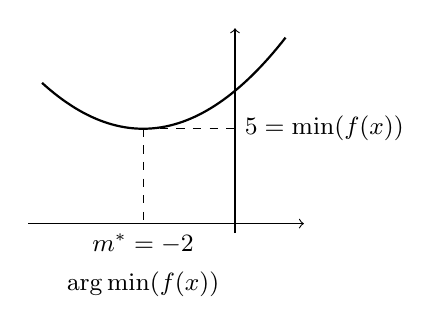
\begin{tikzpicture}
\begin{axis}[
  width=5.2cm, height=4.4cm,
  axis lines=none,
  xmin=-4.6, xmax=1.6, ymin=-1.2, ymax=10.5,
  clip=false]
  \draw[->] (axis cs:-4.5,0) -- (axis cs:1.5,0);
  \draw[->] (axis cs:0,-0.5) -- (axis cs:0,10.3);
  \addplot[thick,domain=-4.2:1.1,samples=60] {0.5*(x+2)^2+5};
  \draw[dashed] (axis cs:-2,5) -- (axis cs:0,5);
  \draw[dashed] (axis cs:-2,5) -- (axis cs:-2,0);
  \node[right,font=\small] at (axis cs:0,5) {$5=\min(f(x))$};
  \node[below,font=\small] at (axis cs:-2,0) {$m^*=-2$};
  \node[font=\small] at (axis cs:-2,-3.2) {$\arg\min(f(x))$};
\end{axis}
\end{tikzpicture}
\qquad\qquad
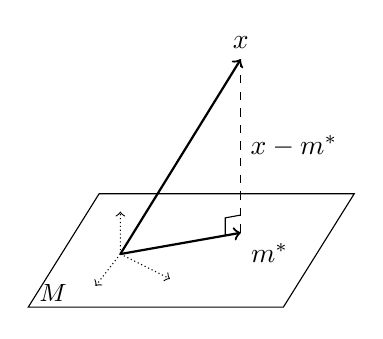
\begin{tikzpicture}[scale=0.9]
  % projection onto plane M
  \draw (0,0) -- (3.6,0) -- (4.6,1.6) -- (1,1.6) -- cycle;
  \node at (0.35,0.2) {\small $M$};
  \coordinate (O) at (1.3,0.75);
  \coordinate (P) at (3.0,1.05);
  \coordinate (X) at (3.0,3.5);
  \draw[->,thick] (O) -- (X) node[above] {$x$};
  \draw[->,thick] (O) -- (P) node[below right] {$m^*$};
  \draw[dashed] (P) -- (X) node[midway,right] {$x-m^*$};
  \draw (3.0,1.3) -- (2.78,1.26) -- (2.78,1.01);
  \draw[->,densely dotted] (O) -- (1.3,1.35);
  \draw[->,densely dotted] (O) -- (0.95,0.3);
  \draw[->,densely dotted] (O) -- (2.0,0.4);
\end{tikzpicture}
\end{center}
Hence:
\begin{itemize}[nosep]
  \item a solution exists;
  \item the solution is unique;
  \item $x-m^*\perp M$.
\end{itemize}

\needspace{14\baselineskip}
\sep
\begin{keybox}[width=0.45\linewidth]
$H = M\overset{\perp}{\oplus} M^\perp, \qquad
x = \underbrace{x_1}_{\in M} + \underbrace{x_2}_{\in M^\perp}$
\end{keybox}
\begin{proof}
For any $m\in M$:
\begin{align*}
\norm{x-m}^2 &= \inner{x-m}{x-m} = \inner{x_1+x_2-m}{x_1+x_2-m}\\
&= \big\langle \underbrace{(\underset{\in M}{x_1}-\underset{\in M}{m})}_{\in M} + \underset{\in M^\perp}{x_2},\; (x_1-m)+x_2 \big\rangle\\
&= \inner{x_1-m}{x_1-m} + \underbrace{\inner{\underset{\in M}{x_1-m}}{\underset{\in M^\perp}{x_2}}}_{0} + \underbrace{\inner{x_2}{x_1-m}}_{0} + \inner{x_2}{x_2}\\
&= \norm{x_1-m}^2 + \norm{x_2}^2\\[4pt]
&\boxed{m^*=x_1} \text{ to minimize this}
\qquad\Longrightarrow\qquad
\boxed{\therefore\ \min \norm{x-m} = \norm{x_2}}
\end{align*}
\begin{itemize}[nosep]
  \item $x_1$ exists;
  \item $x_1$ is unique, as $M\oplus M^\perp$ is a direct sum;
  \item $x-m^* = x-x_1 = x_2\in M^\perp$. \qedhere
\end{itemize}
\end{proof}

\begin{insight}[Why the proof works]
The key identity is the Pythagorean theorem $\norm{x-m}^2 = \norm{x_1-m}^2 + \norm{x_2}^2$, valid because
$x_1-m\in M$ and $x_2\in M^\perp$ are orthogonal. The second term does not depend on $m$, and the first one is
$\ge 0$ with equality \emph{only} for $m=x_1$; this gives existence and uniqueness at once.
The decomposition $H = M\oplus M^\perp$ itself exists because $M$ is finite dimensional: take an orthonormal
basis $\{e_1,\dots,e_k\}$ of $M$ (Gram--Schmidt) and set $x_1=\sum_i \inner{x}{e_i}e_i$, $x_2 = x-x_1$;
then $\inner{x_2}{e_j} = \inner{x}{e_j}-\inner{x}{e_j} = 0$ for every $j$, so $x_2\in M^\perp$.
\end{insight}

\begin{note}
$\V = M^\perp \overset{\perp}{\oplus} M$, \quad $x\in \V$, \quad $x\notin M$.
\[
\R^2 = x\text{ axis} \overset{\perp}{\oplus} y \text{ axis}, \qquad
\R^2 = \underbrace{\Span\left\{\bmat{1\\0}\right\}}_{M} \overset{\perp}{\oplus} \underbrace{\Span\left\{\bmat{0\\1}\right\}}_{M^\perp}
\]
\begin{center}
\begin{tikzpicture}[scale=0.55,baseline=(current bounding box.center)]
  \draw[thick] (-2,0) -- (2.5,0) node[right] {$M$};
  \draw[thick] (0,-2) -- (0,2.5) node[above] {$M^\perp$};
\end{tikzpicture}
\qquad\qquad
$\displaystyle \bmat{1\\2} = \underbrace{\bmat{1\\0}}_{\in M} + \underbrace{\bmat{0\\2}}_{\in M^\perp}$
\end{center}
If a vector is not in $M$, it does not directly mean that it should be inside $M^\perp$. The vector can be written using $M$ and $M^\perp$.
\end{note}

% ===== Page 37 =====
\origpage{37}
\[
x\in M \;\Rightarrow\; m^* = \operatorname{Proj}_M x = x,
\qquad
x = \underbrace{x_1}_{x} + \underbrace{x_2}_{0}: \quad \text{if } x\in M \;\Rightarrow\; \operatorname{Proj}_{M^\perp} x = 0
\]

\begin{example}
$\V=\R^2$, \quad $M=\Span\left\{\bmat{1\\1}\right\}$, \quad $\inner{x}{y} = y\T x$, \quad
$x = \bmat{1\\2}$, \quad $m^* = \operatorname{Proj}_M x$.
\[
m = \alpha\bmat{1\\1} \;\Rightarrow\; m^* = \alpha^*\bmat{1\\1}, \qquad (x-m^*)\perp M
\]
\begin{minipage}[c]{0.56\linewidth}
\begin{align*}
x-m^* = \left(\bmat{1\\2} - \alpha^*\bmat{1\\1}\right) &\perp \bmat{1\\1}\\
\bmat{1-\alpha^*\\ 2-\alpha^*} &\perp \bmat{1\\1}\\
1-\alpha^* + 2-\alpha^* = 0 &\;\Rightarrow\; \alpha^* = \tfrac{3}{2}\\[4pt]
&\boxed{m^* = \frac{3}{2}\bmat{1\\1}}
\end{align*}
\end{minipage}\hfill
\begin{minipage}[c]{0.4\linewidth}
\centering
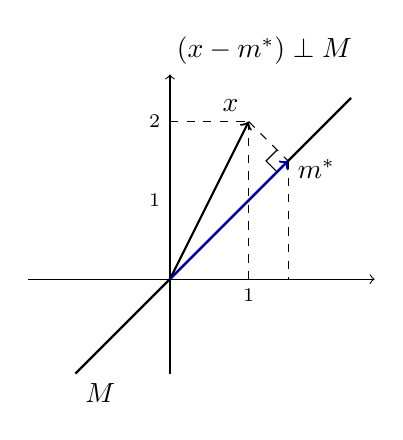
\begin{tikzpicture}[scale=1.0]
  \draw[->] (-1.8,0) -- (2.6,0);
  \draw[->] (0,-1.2) -- (0,2.6);
  \draw[thick] (-1.2,-1.2) -- (2.3,2.3);
  \node[below right] at (-1.2,-1.2) {$M$};
  \node[left] at (0,2) {\scriptsize 2};
  \node[left] at (0,1) {\scriptsize 1};
  \node[below] at (1,0) {\scriptsize 1};
  \draw[->,thick] (0,0) -- (1,2) node[above left] {$x$};
  \draw[dashed] (0,2) -- (1,2);
  \draw[dashed] (1,2) -- (1,0);
  \draw[->,thick,blue!60!black] (0,0) -- (1.5,1.5);
  \node[right] at (1.5,1.4) {$m^*$};
  \draw[dashed] (1,2) -- (1.5,1.5);
  \draw[dashed] (1.5,1.5) -- (1.5,0);
  \draw (1.36,1.36) -- (1.22,1.5) -- (1.36,1.64);
  \node[above] at (1.2,2.6) {$(x-m^*)\perp M$};
\end{tikzpicture}
\end{minipage}
\explain{Check: $x-m^* = \bmat{-1/2 & 1/2}\T$ and $\bmat{-1/2 & 1/2}\bmat{1 & 1}\T = 0$; the distance from $x$ to $M$ is $\norm{x-m^*} = 1/\sqrt2$.}
\end{example}

\begin{example}
Projection onto the span of one or two vectors.

\paragraph{Case 1: one spanning vector.} $\V$, \quad $M=\Span\{v_1\}$.
\[
m^* = \operatorname{Proj}_M x = \,? \qquad m^* = \alpha^* v_1, \qquad x-m^* = (x-\alpha^* v_1)\perp v_1
\]
Hence
\begin{align*}
\inner{x-\alpha^* v_1}{v_1} &= 0\\
\inner{x}{v_1} - \alpha^*\inner{v_1}{v_1} &= 0\\
\Rightarrow\quad \alpha^* &= \frac{\inner{x}{v_1}}{\inner{v_1}{v_1}}, \qquad m^* = \frac{\inner{x}{v_1}}{\inner{v_1}{v_1}}\cdot v_1
\end{align*}

\paragraph{Case 2: two spanning vectors.} $\V$, \quad $M=\Span\{v_1,v_2\}$.
\begin{align*}
m^* &= \operatorname{Proj}_M x = \,?\\
m^* &= \alpha_1^* v_1 + \alpha_2^* v_2\\
(x-\alpha_1^* v_1 - \alpha_2^* v_2)\perp M &\;\Rightarrow\; (x-\alpha_1^* v_1-\alpha_2^* v_2)\perp v_1 \text{ and } v_2
\end{align*}
Taking inner products with $v_1$ and $v_2$:
\begin{align*}
\inner{x-\alpha_1^* v_1-\alpha_2^* v_2}{v_1} = 0 &\;\Rightarrow\; \inner{v_1}{v_1}\alpha_1^* + \inner{v_2}{v_1}\alpha_2^* = \inner{x}{v_1}\\
\inner{x-\alpha_1^* v_1-\alpha_2^* v_2}{v_2} = 0 &\;\Rightarrow\; \inner{v_1}{v_2}\alpha_1^* + \inner{v_2}{v_2}\alpha_2^* = \inner{x}{v_2}
\end{align*}
In matrix form:
\begin{gather*}
\underbrace{\bmat{\inner{v_1}{v_1} & \inner{v_2}{v_1}\\[2pt] \inner{v_1}{v_2} & \inner{v_2}{v_2}}}_{\substack{G\\ \text{Gram matrix}}}
\underbrace{\bmat{\alpha_1^*\\ \alpha_2^*}}_{\alpha^*}
= \underbrace{\bmat{\inner{x}{v_1}\\ \inner{x}{v_2}}}_{b}
\qquad\Longrightarrow\qquad
G\cdot\alpha^* = b, \quad \boxed{\alpha^* = G^{-1}\cdot b}
\end{gather*}

% ===== Page 38 =====
\needspace{5\baselineskip}
The determinant of $G$:\origpage{38}
\begin{align*}
\det G &= \inner{v_1}{v_1}\inner{v_2}{v_2} - \inner{v_1}{v_2}\underbrace{\inner{v_2}{v_1}}_{\overline{\inner{v_1}{v_2}}}\\*
&= \inner{v_1}{v_1}\inner{v_2}{v_2} - \abs{\inner{v_1}{v_2}}^2
\end{align*}
\explain{Cauchy--Schwarz: equality is satisfied if $v_1=\alpha v_2$; only in this case $\det G = 0$.}
Hence
\begin{gather*}
\det G > 0 \quad \text{if } \underbrace{v_1\neq \alpha v_2}_{\text{linearly indep.}}, \qquad
M = \Span\{v_1,v_2\}, \quad m^* = \alpha_1^* v_1 + \alpha_2^* v_2
\end{gather*}
\begin{insight}
By the Cauchy--Schwarz inequality $\abs{\inner{v_1}{v_2}}^2\le\inner{v_1}{v_1}\inner{v_2}{v_2}$, so always
$\det G\ge 0$, with equality iff $v_1,v_2$ are linearly dependent. Hence for a basis $\{v_1,v_2\}$ of $M$ the
system $G\alpha^*=b$ has exactly one solution, which is the unique $m^*$ promised by the projection theorem.
Note also that $G$ is Hermitian: its $(j,i)$ entry is the complex conjugate of its $(i,j)$ entry.
\end{insight}
\end{example}

\begin{example}
$\V = \{f:[0,1]\to\R\}$, \quad $\displaystyle\inner{f}{g} = \int_0^1 f(t)g(t)\,dt$, \quad
$M=\Span\{1,t\}$, \quad $f(t)=t^2$.

Find $m^* = \operatorname{Proj}_M f$, with $v_1(t) = 1$, $v_2(t) = t$:
\begin{align*}
&\underbrace{\bmat{\inner{1}{1} & \inner{t}{1}\\ \inner{1}{t} & \inner{t}{t}}}_{G}\bmat{\alpha_1^*\\ \alpha_2^*} = b = \bmat{\inner{t^2}{1}\\ \inner{t^2}{t}}\\[2pt]
\Rightarrow\ &\bmat{\int_0^1 dt & \int_0^1 t\,dt\\[4pt] \int_0^1 t\,dt & \int_0^1 t^2\,dt}\bmat{\alpha_1^*\\ \alpha_2^*} = \bmat{\int_0^1 t^2\,dt\\[4pt] \int_0^1 t^3\,dt}\\[2pt]
\Rightarrow\ &\underbrace{\bmat{1 & 1/2\\ 1/2 & 1/3}}_{G}\bmat{\alpha_1^*\\ \alpha_2^*} = \bmat{1/3\\ 1/4},
\qquad \det G = \frac13 - \frac14 = \frac1{12}\\[2pt]
&\bmat{\alpha_1^*\\ \alpha_2^*} = \frac{1}{\frac{1}{12}}\bmat{1/3 & -1/2\\ -1/2 & 1}\bmat{1/3\\ 1/4} = \bmat{-1/6\\ 1}
\end{align*}
\begin{gather*}
\boxed{m^* = \operatorname{Proj}_M f = -\frac16 + t}\\[4pt]
\norm{f(t)} = \sqrt{\int_0^1 \abs{f(t)}^2\,dt}, \qquad
\min_{m\in M} \norm{\underbrace{t^2}_{x} - m(t)} =
\min_{m(t)\in M} \sqrt{\int_0^1 \abs{t^2-m(t)}^2\,dt}
\end{gather*}
% note: the "=" between the two minimizations is added for readability (in the notes they are written side by side)
\needspace{14\baselineskip}
\begin{center}
\begin{tikzpicture}
\begin{axis}[
  width=6.5cm, height=5.5cm,
  axis lines=middle,
  xmin=-0.15, xmax=1.35, ymin=-0.3, ymax=1.4,
  xtick={1}, ytick={1},
  tick label style={font=\scriptsize},
  clip=false]
  \fill[gray!30] (axis cs:0,0) -- plot[domain=0:1,samples=40] (axis cs:\x,{\x*\x}) -- plot[domain=1:0,samples=2] (axis cs:\x,{\x-1/6}) -- cycle;
  \addplot[thick,domain=0:1.1,samples=60] {x^2};
  \addplot[thick,red!60!black,domain=0:1.2,samples=2] {x-1/6};
  \addplot[thick,blue!60!black,domain=0:1,samples=2] {x};
  \draw[densely dotted] (axis cs:0,1) -- (axis cs:1,1);
  \draw[dashed] (axis cs:1,1) -- (axis cs:1,0);
  \node[above left,blue!60!black] at (axis cs:0.45,0.45) {$t$};
  \node[right,red!60!black] at (axis cs:1.2,1.2-1/6) {$m^*=t-\tfrac16$};
  \node[above] at (axis cs:1.1,1.21) {$x=t^2$};
  \node[below left,font=\scriptsize] at (axis cs:0,0) {$0$};
\end{axis}
\end{tikzpicture}
\end{center}
\explain{Shaded: the gap between $t^2$ and its best approximation $m^*$ in $\Span\{1,t\}$.}
\begin{insight}[Checking the answer]
The error $e(t) = t^2-t+\tfrac16$ must be orthogonal to $1$ and $t$:
\begin{align*}
\inner{e}{1} &= \int_0^1 \big(t^2-t+\tfrac16\big)\,dt = \tfrac13-\tfrac12+\tfrac16 = 0,\\
\inner{e}{t} &= \int_0^1 \big(t^3-t^2+\tfrac16 t\big)\,dt = \tfrac14-\tfrac13+\tfrac1{12} = 0. \quad\checkmark
\end{align*}
Since $e\perp m^*$, the minimum error is
\begin{gather*}
\norm{e}^2 = \inner{e}{t^2} = \tfrac15-\tfrac14+\tfrac1{18} = \tfrac1{180},
\qquad\text{i.e.}\qquad
\min_{m\in M}\norm{t^2-m} = \tfrac{1}{6\sqrt5}\approx 0.075.
\end{gather*}
So $t-\tfrac16$ is the best straight-line
(least-squares) fit to $t^2$ on $[0,1]$; it crosses $t^2$ at $t=\tfrac12\pm\tfrac{1}{2\sqrt3}$.
\end{insight}
\end{example}

% ===== Page 39 =====
\subsection{Computing Projections: the Gram Matrix and Normal Equations}\label{ss:gram}
\paragraph{General space.}
$\V$,\origpage{39} $n$ dimensional, \quad $M = \Span\{\underbrace{v_1,v_2,\dots,v_k}_{\text{linearly indep.}}\}$, \quad $k<n$.
\[
m^* = \sum_{i=1}^k \alpha_i^* v_i,
\qquad
x-m^* = x-\sum_{i=1}^k \alpha_i^* v_i \;\perp\; v_1, v_2, \dots, v_k
\]
Taking inner products with each $v_j$:
\begin{align*}
\Big\langle x-\sum_{i=1}^k \alpha_i^* v_i,\, v_j\Big\rangle &= 0, \qquad j=1,2,\dots,k\\
\inner{x}{v_j} - \sum_{i=1}^k \alpha_i^*\inner{v_i}{v_j} &= 0
\end{align*}
In matrix form:
\begin{gather*}
\underbrace{\bmat{\inner{v_1}{v_1} & \cdots & \inner{v_k}{v_1}\\ \vdots & \ddots & \vdots\\ \inner{v_1}{v_k} & \cdots & \inner{v_k}{v_k}}}_{G}
\underbrace{\bmat{\alpha_1^*\\ \vdots\\ \alpha_k^*}}_{\alpha^*}
= \underbrace{\bmat{\inner{x}{v_1}\\ \vdots\\ \inner{x}{v_k}}}_{b}
\end{gather*}
\key{$G$ is invertible iff $v_1,\dots,v_k$ are linearly independent}, and then $\alpha^* = G^{-1}b$.
\explain{These $k$ equations are the \term{normal equations}; $G$ is the \term{Gram matrix}. $G$ is Hermitian and positive definite for independent $v_i$:
$\beta\Hm G\beta = \norm{\textstyle\sum_i\beta_i v_i}^2 > 0$ for $\beta\neq0$ (written for $\F=\C$ with $G_{ji}=\inner{v_i}{v_j}$).}

\paragraph{Specific case: orthogonal basis.}
$v_i\perp v_j$ when $i\neq j$: \quad $\{v_1,\dots,v_k\}$ are orthogonal, so $G$ is diagonal:
\begin{gather*}
\bmat{\inner{v_1}{v_1} & & & 0\\ & \inner{v_2}{v_2} & & \\ & & \ddots & \\ 0 & & & \inner{v_k}{v_k}}
\bmat{\alpha_1^*\\ \vdots\\ \alpha_k^*} = \bmat{\inner{x}{v_1}\\ \vdots\\ \inner{x}{v_k}}\\[6pt]
G^{-1}b = \bmat{\dfrac{1}{\inner{v_1}{v_1}} & & 0\\ & \ddots & \\ 0 & & \dfrac{1}{\inner{v_k}{v_k}}}
\bmat{\inner{x}{v_1}\\ \vdots\\ \inner{x}{v_k}}
= \bmat{\dfrac{\inner{x}{v_1}}{\inner{v_1}{v_1}}\\ \vdots\\ \dfrac{\inner{x}{v_k}}{\inner{v_k}{v_k}}}\\[6pt]
\alpha_i^* = \frac{\inner{x}{v_i}}{\inner{v_i}{v_i}}, \qquad
\boxed{m^* = \sum_{i=1}^k \frac{\inner{x}{v_i}}{\inner{v_i}{v_i}}\cdot v_i}
\end{gather*}
For an orthonormal set ($v_i\perp v_j$, $i\neq j$, and $\norm{v_i}=1$):
\begin{gather*}
\boxed{m^* = \sum_{i=1}^k \inner{x}{v_i}\, v_i}
\end{gather*}

\begin{example}
$\V = \R^{2\times 2}$, \quad $M = \{\text{set of symmetric matrices}\}$
\[
x = \bmat{a & b\\ c & d}, \qquad m^* = \operatorname{Proj}_M x, \qquad \inner{A}{B} = \tr(A\T B)
\]
For $2\times 2$ matrices:
\begin{align*}
\tr\left(\bmat{a_{11} & a_{21}\\ a_{12} & a_{22}}\bmat{b_{11} & b_{12}\\ b_{21} & b_{22}}\right)
&= \tr\left(\bmat{a_{11}b_{11}+a_{21}b_{21} & \times\\ \times & a_{12}b_{12}+a_{22}b_{22}}\right)\\
&= a_{11}b_{11} + a_{21}b_{21} + a_{12}b_{12} + a_{22}b_{22}\\[4pt]
\norm{A} &= \sqrt{\tr(A\T A)} = \sqrt{\inner{A}{A}}
\end{align*}
% ===== Page 40 =====
We look for\origpage{40}
\begin{gather*}
\min_{S\ \text{sym.}} \Big(\tr\big[(x-S)\T(x-S)\big]\Big)^{1/2}\\[4pt]
M = \Span\Big\{\underbrace{\bmat{1&0\\0&0}}_{v_1},\ \underbrace{\bmat{0&1\\1&0}}_{v_2},\ \underbrace{\bmat{0&0\\0&1}}_{v_3}\Big\}
\end{gather*}
% corrected: notes had the third label as v_2 (meant v_3)
\explain{$v_1,v_2,v_3$ are mutually orthogonal (no common nonzero entries), so the orthogonal-basis formula $\alpha_i^* = \inner{x}{v_i}/\inner{v_i}{v_i}$ applies.}
Hence
\begin{alignat*}{2}
\inner{x}{v_1} &= a, &\qquad \inner{v_1}{v_1} &= 1\\
\inner{x}{v_2} &= b+c, &\qquad \inner{v_2}{v_2} &= 2\\
\inner{x}{v_3} &= d, &\qquad \inner{v_3}{v_3} &= 1
\end{alignat*}
and
\begin{align*}
m^* &= a\bmat{1&0\\0&0} + \frac{b+c}{2}\bmat{0&1\\1&0} + d\bmat{0&0\\0&1}
= \bmat{a & \frac{b+c}{2}\\ \frac{b+c}{2} & d} = \frac{x+x\T}{2}\\
\operatorname{Proj}_{M^\perp} x &= x-m^* = x - \left(\frac{x+x\T}{2}\right) = \frac{x-x\T}{2}\\[4pt]
&\left.\begin{aligned} M &\to 3\text{ dim.}\\ M^\perp &\to 1\text{ dim.}\end{aligned}\right\} \;\V \Rightarrow 4\text{ dim.}
\end{align*}
\begin{insight}
$M^\perp$ is the set of \key{skew-symmetric} matrices, $M^\perp = \Span\{K_0\}$ with $K_0 = \bmat{0&1\\-1&0}$:
for $S=S\T$ and $K=-K\T$,
\[
\inner{K}{S} = \tr(S\T K) = \tr(SK) = \tr\big((SK)\T\big) = \tr(K\T S) = -\tr(KS) = -\tr(SK),
\]
so $\inner{K}{S}=0$. Thus every square matrix splits uniquely as
\[
x = \underbrace{\tfrac{x+x\T}{2}}_{\text{symmetric}} + \underbrace{\tfrac{x-x\T}{2}}_{\text{skew-symmetric}},
\]
and $\tfrac{x+x\T}{2}$ is the symmetric matrix closest to $x$ in the Frobenius norm $\sqrt{\tr(A\T A)}$.
\end{insight}
\end{example}

\needspace{16\baselineskip}
\subsection{Orthogonal Projections in $\C^n$: Projection Matrices}\label{ss:proj-matrices}
$\V=\C^n$, \quad $M = \Span\{m_1,\dots,m_k\}$, \quad $m_i = [\ \ ] \in\C^n$ (column vectors), \quad $x\in\C^n$.
\begin{align*}
m^* &= \operatorname{Proj}_M x = \,?\\
m^* &= P_M\cdot x \quad\Rightarrow\quad P_M\text{: \term{projection matrix} onto } M.
\end{align*}
Writing $m^*$ in terms of the spanning vectors:
\begin{gather*}
m^* = \alpha_1^* m_1 + \alpha_2^* m_2 + \dots + \alpha_k^* m_k
= \underbrace{\big[\, m_1 \,\vdots\, m_2 \,\vdots\, \cdots \,\vdots\, m_k\,\big]}_{B}
\underbrace{\bmat{\alpha_1^*\\ \alpha_2^*\\ \vdots\\ \alpha_k^*}}_{\alpha^*}\\[4pt]
m^* = B\alpha^*, \qquad x-B\alpha^* \perp m_1, m_2, \dots, m_k, \qquad \inner{x}{y} = y\Hm x
\end{gather*}
% note: "<x,y> = y^H x" is written twice in the notes
Hence
\begin{align*}
\inner{x-B\alpha^*}{m_j} = 0 \quad\Leftrightarrow\quad & m_j\Hm(x-B\alpha^*) = 0 \quad\forall j\\
& m_1\Hm(x-B\alpha^*) = 0\\
& \quad\vdots\\
& m_k\Hm(x-B\alpha^*) = 0
\end{align*}
Stacking these $k$ equations:
\begin{gather*}
\underbrace{\bmat{m_1\Hm\\ \hline \rule{0pt}{2.8ex}m_2\Hm\\ \hline \rule{0pt}{2.8ex}\vdots\\ \hline \rule{0pt}{2.8ex}m_k\Hm}}_{B\Hm}(x-B\alpha^*) = 0
\qquad\Longrightarrow\qquad
\begin{aligned}
B\Hm(x-B\alpha^*) &= 0\\
B\Hm x - B\Hm B\alpha^* &= 0\\
\underbrace{B\Hm B}_{G}\,\alpha^* &= \underbrace{B\Hm x}_{b}
\end{aligned}
\end{gather*}

% ===== Page 41 =====
Indeed,\origpage{41}
\begin{gather*}
\underbrace{\bmat{m_1\Hm\\ \vdots\\ m_k\Hm}}_{B\Hm}
\underbrace{\big[\, m_1 \,\vdots\, m_2 \,\vdots\, \cdots \,\vdots\, m_k\,\big]}_{B}
= \bmat{m_1\Hm m_1 & \cdots & m_1\Hm m_k\\ \vdots & \ddots & \vdots\\ m_k\Hm m_1 & \cdots & m_k\Hm m_k}
= \underbrace{\bmat{\inner{m_1}{m_1} & \cdots & \inner{m_k}{m_1}\\ \vdots & \ddots & \vdots\\ \inner{m_1}{m_k} & \cdots & \inner{m_k}{m_k}}}_{G}\\[6pt]
B\Hm x = \bmat{m_1\Hm x\\ m_2\Hm x\\ \vdots\\ m_k\Hm x} = \bmat{\inner{x}{m_1}\\ \inner{x}{m_2}\\ \vdots\\ \inner{x}{m_k}} = b
\end{gather*}
% corrected: notes had "B x^H = [m_i^H x] = [<x,m_i>] = [Gram matrix]". B x^H is B^H x, and the Gram matrix
% belongs to B^H B (entry (i,j) = m_i^H m_j = <m_j,m_i>), so it was moved to the line above.
\explain{So $B\Hm B\,\alpha^* = B\Hm x$ is exactly the Gram system $G\alpha^* = b$ of the general case, with $\inner{x}{y}=y\Hm x$.}
Solving for $\alpha^*$:
\begin{align*}
\alpha^* &= (B\Hm B)^{-1}B\Hm x\\
m^* &= B\alpha^*\\
m^* &= \operatorname{Proj}_M x = B(B\Hm B)^{-1}B\Hm x\\[4pt]
&\boxed{P_M = B(B\Hm B)^{-1}B\Hm}, \qquad m^* = P_M x
\end{align*}
\needspace{5\baselineskip}
For the orthogonal complement:
\begin{align*}
P_{M^\perp} &= I-P_M\\
\operatorname{Proj}_{M^\perp} x &= x-\operatorname{Proj}_M x\\
&= x - P_M x = (I-P_M)x
\end{align*}
% corrected: notes had "P_{M^perp} = (I-P_M) x" (the matrix is I-P_M; (I-P_M)x is the projected vector)

\needspace{8\baselineskip}
\sep
Properties of $P_M$:
\begin{align*}
P_M\Hm &= \big(B(B\Hm B)^{-1}B\Hm\big)\Hm = B\big((B\Hm B)^{-1}\big)\Hm B\Hm = B(B\Hm B)^{-1}B\Hm = P_M\\
&\Rightarrow\ P_M\Hm = P_M\\
P_M^2 &= P_M\cdot P_M\\
P_M^2 &= B(B\Hm B)^{-1}\cancel{B\Hm B}\,\cancel{(B\Hm B)^{-1}}B\Hm = B(B\Hm B)^{-1}B\Hm = P_M\\[4pt]
&\boxed{P_M^2 = P_M}
\end{align*}
% corrected: notes had "B(B^H B^{-1})B^H" in the last step; it is B(B^H B)^{-1}B^H
\explain{$(B\Hm B)^{-1}$ is Hermitian because $B\Hm B$ is: $\big((B\Hm B)^{-1}\big)\Hm = \big((B\Hm B)\Hm\big)^{-1} = (B\Hm B)^{-1}$.}
\begin{center}
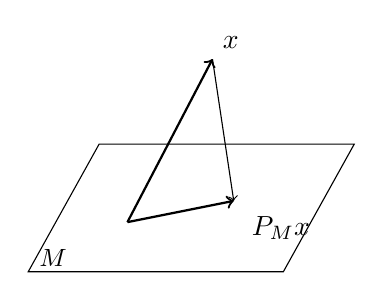
\begin{tikzpicture}[scale=0.9,baseline=(current bounding box.center)]
  \draw (0,0) -- (3.6,0) -- (4.6,1.8) -- (1,1.8) -- cycle;
  \node at (0.35,0.2) {\small $M$};
  \coordinate (O) at (1.4,0.7);
  \coordinate (P) at (2.9,1.0);
  \coordinate (X) at (2.6,3.0);
  \draw[->,thick] (O) -- (X) node[above right] {$x$};
  \draw[->,thick] (O) -- (P);
  \node[below right,xshift=3pt,yshift=-2pt] at (P) {$P_M x$};
  \draw[->] (X) -- (P);
\end{tikzpicture}
\qquad\qquad
$\begin{aligned}
&P_M\cdot P_M x = P_M x\\
&\underline{P_M^2 x = P_M x}
\end{aligned}$
\end{center}

\begin{remark}
An \term{orthogonal projection matrix} $P\in\C^{n\times n}$ satisfies
\begin{enumerate}[label=\roman*-), nosep]
  \item $P\Hm = P$
  \item $P^2 = P$ \quad ($P^k = P$ for every $k\ge 1$)
\end{enumerate}
Also,
\begin{align*}
(I-P)^2 &= I-P\\
(I-P)(I-P) &= I-\cancel{P}-P+\overbrace{P^2}^{\cancel{P}}\\
&= I-P
\end{align*}
\end{remark}
\begin{insight}[Remarks on $P_M$]
\begin{itemize}[nosep]
  \item Conversely, \key{any $P$ with $P\Hm=P$ and $P^2=P$ is the orthogonal projection onto $\Range(P)$}:
        $x = Px + (I-P)x$ with $Px\in\Range(P)$, and $(I-P)x\perp\Range(P)$ because
        \[
        (Py)\Hm(I-P)x = y\Hm(P-P^2)x = 0 \qquad\text{for all } y.
        \]
  \item \key{$P_M$ depends only on $M$}, not on the chosen basis: if $B' = BT$ with $T$ invertible, then
        $B'(B'^H B')^{-1}B'^H = BT\,T^{-1}(B\Hm B)^{-1}T^{-H}\,T\Hm B\Hm = P_M$.
  \item If the columns of $B$ are orthonormal, $B\Hm B = I$ and $P_M = BB\Hm = \sum_i m_i m_i\Hm$,
        which is the matrix form of $m^* = \sum_i\inner{x}{m_i}m_i$.
  \item $P_M m = m$ for $m\in M$ and $P_M y = 0$ for $y\in M^\perp$ (since $B\Hm y = 0$);
        hence $\Range(P_M) = M$, $\Null(P_M) = M^\perp$.
\end{itemize}
\end{insight}

% ===== Page 42 =====
\begin{example}
$\V=\R^3$,\origpage{42} \quad $M = \Span\left\{\bmat{1\\1\\1},\bmat{1\\-1\\1}\right\}$, \quad
$x = \bmat{1\\0\\0}$. \quad Find $\operatorname{Proj}_M x = \,?$
\begin{gather*}
B = \bmat{1&1\\1&-1\\1&1}, \qquad
B\Hm B = B\T B = \bmat{1&1&1\\1&-1&1}\bmat{1&1\\1&-1\\1&1} = \bmat{3&1\\1&3},\\[4pt]
(B\Hm B)^{-1} = \bmat{3&-1\\-1&3}\cdot\frac18
\end{gather*}
Then
\begin{align*}
\operatorname{Proj}_M x &= B(B\Hm B)^{-1}B\Hm x = P_M x\\
&= \frac18\bmat{1&1\\1&-1\\1&1}\bmat{3&-1\\-1&3}\underbrace{\bmat{1&1&1\\1&-1&1}\bmat{1\\0\\0}}_{\bmat{1\\1}}\\
&= \frac18\bmat{1&1\\1&-1\\1&1}\underbrace{\bmat{3&-1\\-1&3}\bmat{1\\1}}_{\bmat{2\\2}}\\
&= \frac18\cdot\bmat{4\\0\\4} = \bmat{1/2\\0\\1/2}\\[4pt]
x-\operatorname{Proj}_M x &= \bmat{1\\0\\0} - \bmat{1/2\\0\\1/2} = \bmat{1/2\\0\\-1/2}
\end{align*}
% note: in the notes the three products are shown as nested underbraces under one line
\explain{This difference should be orthogonal to the basis vectors (``sağlaması için kullanılabilir'' --- can be used to check the result).}
% Turkish: "can be used to verify (the result)"
\explain{Check, and the full projection matrix (its first column is indeed $\operatorname{Proj}_M x$):}
\begin{gather*}
\bmat{1&1&1}\bmat{1/2\\0\\-1/2} = 0, \qquad \bmat{1&-1&1}\bmat{1/2\\0\\-1/2} = 0 \quad\checkmark\\*[4pt]
P_M = \frac18 B\bmat{3&-1\\-1&3}B\T = \frac12\bmat{1&0&1\\0&2&0\\1&0&1}
\end{gather*}
\end{example}
